\documentclass[11pt]{article}

% Settings to be used with dvips followed by ps2pdf
\usepackage[dvips,
    pdftitle={TVLA User Manual},
    pdfauthor={Roman Manevich and Mooly Sagiv},
    pdfsubject={TVLA User Manual},
    hyperindex,
    backref,
    hyperfigures,
    colorlinks,
    bookmarks,
    bookmarksnumbered,
    bookmarksopen,
    citecolor=blue,
    urlcolor=blue,
    pdfstartview={FitH}
]{hyperref}

\usepackage{amsmath,alltt,epsfig}

\newcommand{\otherwise}{\makebox{{\rm otherwise}}}
\newcommand{\secref}[1]{Section~\ref{Se:#1}}
\newcommand{\lemref}[1]{Lemma~\ref{Lm:#1}}
\newcommand{\figref}[1]{Figure~\ref{Fi:#1}}
\newcommand{\defref}[1]{Definition~\ref{De:#1}}
\renewcommand{\eqref}[1]{(\ref{Eq:#1})}
\newcommand{\tableref}[1]{Table~\ref{Ta:#1}}
\newcommand{\subsubsubsection}[1]{\emph{#1}:}
\newcommand{\tn}{{\texttt n}}
\newcommand{\tx}{{\texttt x}}
\newcommand{\ty}{{\texttt y}}
\newcommand{\ttt}{{\texttt t}}
\newcommand{\td}{{\texttt d}}
\newcommand{\tw}{{\texttt w}}
\newcommand{\tL}{{\texttt L}}
\newcommand{\tvexists}[1]{\exists #1:\/}
\newcommand{\tvforall}[1]{\forall #1:\/}
\newcommand{\tvand}{\land}
\newcommand{\tvor}{\lor}
\newcommand{\tvstar}{^*}
\newcommand{\tvplus}{^+}
\newcommand{\tvneq}{\neq}
\newcommand{\tvneg}{\neg}
\newcommand{\tvtype}{\bf \%types}
\newcommand{\tveq}{=}
\newcommand{\impliesT}{\ \makebox{$\triangleright$}\ }
\newcommand{\seq}{\boldsymbol{=}}
\newcommand{\nseq}{\boldsymbol{\neq}}
\newcommand{\sqsupseteqt}{\rhd}
\newcommand{\TRUE}{\boldsymbol{1}}
\newcommand{\FALSE}{\boldsymbol{0}}
\newcommand{\UNKNOWN}{\boldsymbol{1/2}}
\newcommand{\TC}[5]{(\mbox{{\it TC\/}}~{#1, #2}: #3)(#4, #5)}
\newcommand{\threeValue}[3]{{\lsyn #1 \rsyn^{#2}(#3)}}
\newcommand{\evaluate}[3]{{\lsyn #1 \rsyn^{#2}(#3)}}
\newcommand{\twoValue}[3]{\lsyn{#1}\rsyn_2^{#2}(#3)}
\newcommand{\lt}{$<$}
\newcommand{\gt}{$>$}
\newcommand{\deref}{\makebox{{\tt ->}}}
\newcommand{\PVar}{{\it PVar}}
\newcommand{\param}[1]{$<$#1$>$}
\newcommand{\freeVars}{{\it freeVars\/}}
\newcommand{\closure}{{\it closure\/}}
\newcommand{\blur}{{\it blur\/}}
\newcommand{\coerce}{{\it Coerce\/}}
\newcommand{\foreach}{\textbf{foreach}}
\newcommand{\predbox}{\textbf{box}}
\newcommand{\foreachI}{\textbf{for}\=\+\textbf{each}}
\newcommand{\unique}{\textbf{unique}}
\newcommand{\function}{\textbf{function}}
\newcommand{\invfunction}{\textbf{invfunction}}
\newcommand{\symmetric}{\textbf{symmetric}}
\newcommand{\antisymmetric}{\textbf{antisymmetric}}
\newcommand{\reflexive}{\textbf{reflexive}}
\newcommand{\antireflexive}{\textbf{antireflexive}}
\newcommand{\transitive}{\textbf{transitive}}
\newcommand{\tvmessage}{\textbf{\%message}}
\newcommand{\tvmessageI}{\textbf{\%m}\=\+\textbf{essage}}
\newcommand{\tvset}{\textbf{\%s}}
\newcommand{\tvtypes}{\textbf{\%types}}
\newcommand{\predicate}{\textbf{\%p}}
\newcommand{\instrum}{\textbf{\%i}}
\newcommand{\inset}{\textbf{in}}
\newcommand{\constraint}{\textbf{\%r}}
\newcommand{\action}{\textbf{\%action}}
\newcommand{\actionI}{\textbf{\%ac}\=\+\textbf{tion}}
\newcommand{\focus}{\textbf{\%f}}
\newcommand{\precond}{\textbf{\%p}}
\newcommand{\new}{\textbf{\%new}}
\newcommand{\retain}{\textbf{\%retain}}
\newcommand{\tvtitle}{\textbf{\%t}}
\newcommand{\seperator}{\textbf{\%\%}}
\newcommand{\tvimpl}{\rightarrow}
\newcommand{\STRUCT}[1]{\mbox{3-STRUCT}[#1]}
\newcommand{\Voc}{{\cal P}}
\newcommand{\bod}{\textbf{od}}
\newcommand{\bfor}{\textbf{for}}
\newcommand{\bdo}{\textbf{do}}
\newcommand{\breturn}{\textbf{return}}
\newcommand{\bif}{\textbf{if}}
\newcommand{\bthen}{\textbf{then}}
\newcommand{\belse}{\textbf{else}}
\newcommand{\bfi}{\textbf{fi}}
\newcommand{\bwhile}{\textbf{while}}
\newcommand{\bwhileI}{\textbf{wh}\=\+\textbf{ile}}
\newcommand{\authorText}[1]{{\textbf{#1}}} 

\begin{document}

\hfuzz 2pt % Don't bother to report over-full boxes if over-edge is < 2pt
\textheight 20cm

\title{TVLA 3: User's Manual\\(Working Draft)}

\author{Tal Lev-Ami\thanks{\url{mailto:tla@post.tau.ac.il}}
\and Roman Manevich\thanks{\url{mailto:roman.manevich@cs.tau.ac.il}} \and
Mooly Sagiv\thanks{\url{mailto:msagiv@post.tau.ac.il}}}

\maketitle

\tableofcontents

\newpage
\section{Introduction}

This document is intended as a user's manual for the TVLA system.
The reader should be familiar with the Three-Valued Logic based
Analysis framework described in~\cite{TOPLAS:SRW02} before
consulting this manual.  The manual is accompanied by an example
of the analysis of the reverse function in \figref{Reverse}.

The original algorithms in the system were designed and implemented
by Tal Lev-Ami~\cite{kn:TalSAS00,Master:LevAmi00}.

\subsection{Downloading and installing}

The system and latest information is available at:\\
\url{http://www.cs.tau.ac.il/~tvla/}.\\
Please see the file LICESNE for licensing information.

Installation procedure:
\begin{enumerate}
\item TVLA is written in Java and requires J2SE version 1.6 (or
above), available from \url{http://java.sun.com/j2se/}. Before
attempting to run TVLA, make sure it is possible to launch Java
executables by entering ``java'' at the command-line prompt.

\item TVLA uses DOT to generate Postscript files and requires
Graphviz version 2.24 (or above), available from\\
\url{http://www.research.att.com/sw/tools/graphviz/}.  After
installing Graphviz, make sure the bin sub-directory is added to
your path.

\item Extract the archive's content and set the environment
variable TVLA\_HOME to that location.

\item Add the bin sub-directory to your path (the bin directory
contains running scripts for Windows and Linux).

\textbf{IMPORTANT:} Make sure the path does not contain trailing
'$\backslash$' characters or trailing `/` characters.

\item You are now ready to run the system.  Enter tvla to see
usage information and command-line options.
\end{enumerate}

%\subsection{Summary of this document}

\begin{figure}
\begin{center}
\framebox{
\begin{tabular}{@{\hspace{1ex}}c@{\hspace{1ex}}c@{\hspace{1ex}}}
\begin{minipage}{1in}
\begin{alltt}
\begin{tabbing}
/* list.h */ \\
ty\=pedef struct node \\
\{\+\\
        struct node *n;  \\
        int data;      \- \\
\} *L;
\end{tabbing}
\end{alltt}
\end{minipage}
&
\begin{minipage}{1in}
\begin{alltt}
\begin{tabbing}
/* reverse.c */ \\
\#include "list.h" \\
L re\=verse(L x) \{ \+ \\
     L y, t; \\
     y = NULL; \\
     whil\=e (x != NULL) \{ \+ \\
           t = y; \\
           y = x; \\
           x = x->n; \\
           y->n = t; \\
           t = NULL; \- \\
     \} \\
     return y; \- \\
\}
\end{tabbing}
\end{alltt}
\end{minipage}
\\
(a) & (b)
\end{tabular}}
\end{center}
\caption{\label{Fi:Reverse}(a)~Declaration of a linked-list data
type in C. (b)~A C function that uses destructive updating to
reverse the list pointed to by parameter \tx.}
\end{figure}

\section{Graphical representation}

$3$-valued structures are displayed using graphical
representation. For example an input structure for the reverse
function is given in \figref{ManReverseTVS}.

\begin{figure}
\begin{center}
\begin{minipage}[t]{.33\linewidth}
%\vspace*{4cm}
\begin{tabbing}
\%n = \{head, tail\}\\
\%p =\=\+\ \{\\
      sm = \{tail:1/2\}\\
      n = \{head\deref tail:1/2, tail\deref tail:1/2\}\\
      x = \{head\}\\
      t[n] = \{head\deref head, head\deref tail, tail\deref tail:1/2\}\\
      r[n,x] = \{head, tail\}\-\\
\}
\end{tabbing}
\end{minipage}\hfill
\begin{minipage}[t]{.33\linewidth}
\vspace*{0mm} 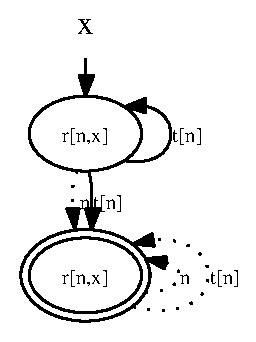
\epsfig{file=sll_tvs,width=3cm}
\end{minipage}
\end{center}
\caption{\label{Fi:ManReverseTVS}The TVS of an input structure for
the reverse function analysis and its graphical representation.}
\end{figure}

\subsection{Colors}

Colors are used to represent the different values for predicates.
Solid black is true ($1$), dotted black is unknown ($1/2$), and
red is false ($0$).

\subsection{Shapes}

The values of nullary predicates are displayed in a box titled
``nullary''.  By default, nullary predicates with true values are
written inside the box, nullary predicates with false values, are
not shown and nullary predicates with indefinite values ($1/2$)
have the value added next to them.

An ellipse represents a node.  If the ellipse is double-circled
then the node is a summary node, and if it is green then the node
is maybe active ($ac=1/2$).  Unary predicates are written within
the ellipse.  If the value is different from $1$ it is appended to
predicate's name (i.e., $=0$ or $=1/2$).


\subsection{Edges}

Binary predicates are represented as directed arrows between the
left and right arguments and annotated by the name of the
predicate.  If a binary predicate has the same value for both
$u_1\deref u_2$ and $u_2\deref u_1$ the two edges are replaced
with a bidirectional edge.

\section{\label{Se:TVPMan}TVP}

\renewcommand{\impliesT}{\ \makebox{\tt ==>}\ }
\newcommand{\blp}{$\boldsymbol{(}$}
\newcommand{\brp}{$\boldsymbol{)}$}
\newcommand{\blcb}{\textbf{\{}}
\newcommand{\brcb}{\textbf{\}}}
\newcommand{\blb}{$\boldsymbol{[}$}
\newcommand{\brb}{$\boldsymbol{]}$}
\newcommand{\lb}{$[$}
\newcommand{\rb}{$]$}
\newcommand{\bor}{{\bf {\tt |}}}
\newcommand{\band}{\textbf{\&}}
\newcommand{\beq}{\textbf{==}}
\newcommand{\bassign}{\textbf{=}}
\newcommand{\bnot}{\textbf{!}}
\newcommand{\bneq}{\textbf{!=}}
\newcommand{\bcomma}{\textbf{,}}
\newcommand{\pformula}{\param{formula}}
\newcommand{\pvar}{\param{var}}
\newcommand{\var}{\param{var}}
\newcommand{\pid}{\param{id}}
\newcommand{\ppred}{\param{pred}}
\newcommand{\csep}[1]{#1$\bowtie$\bcomma}
\newcommand{\nvars}{\blp\ \csep{\var}\ \brp}
\newcommand{\twovars}{\blp\ \var\ \bcomma\ \var\ \brp}

\renewcommand{\tvexists}[1]{\makebox{E($#1$) }}
\renewcommand{\tvforall}[1]{\makebox{A($#1$) }}
\renewcommand{\tvand}{\makebox{ $\&$ }}
\renewcommand{\tvor}{\makebox{ $|$ }}
\renewcommand{\tvstar}{\makebox{$*$}}
\renewcommand{\tvplus}{\makebox{$+$}}
\renewcommand{\tvneq}{\makebox{ $!=$ }}
\renewcommand{\tvneg}{\makebox{ $!$ }}
\renewcommand{\tveq}{\makebox{ $==$ }}

\begin{figure}
\framebox{
\begin{minipage}{1in}
\begin{tabbing}
// Set of names of program variables.\\
\tvset\ PVar\ \{x, y, t\}\\
/* Program variables definition */\\
\foreach\ \= (z \inset\ Var)  \{\+ \\
 \predicate\ $z(v1)$ unique pointer
 \- \\
\}\\
// A predicate to represent the n field of the list data type.\\
\predicate\ $n(v1, v2)$ function
\\
// Is shared instrumentation.\\
\instrum\ $is[n](v) = \tvexists{v1, v2} (v1 \tvneq v2 \tvand n(v1, v) \tvand n(v2, v))$\\
// Reachability instrumentation.\\
\foreach\ (z \inset\ PVar) \{
\instrum\ $r[n,z](v) =\tvexists{v1} (z(v1) \tvand n\tvstar(v1, v))$ \}\\
// The t[n] predicate records transitive reflexive reachability between\\
// list elements along the n field.\\
\instrum\ $t[n](v1, v2) = n*(v1, v2)$ transitive reflexive\\
// Cyclicity instrumentation.\\
\instrum\ $c[n](v) = n\tvplus(v, v)$
\end{tabbing}
\end{minipage}
}
\caption{\label{Fi:ManRevDecl}The declarations part of the TVP for the reverse
function shown in \figref{Reverse}.}
\end{figure}

\begin{figure}
\framebox{
\begin{minipage}{1in}
\begin{tabbing}
/******************************** Generic Actions *****************************/\\
\actionI\  Is\_Not\_Null\_Var(x1) \{
    \tvtitle\  x1 + " != NULL"\\
    \focus\  \{ $x1(v)$ \}
    \precond\  $\tvexists{v} x1(v)$\-\\
\}\\
\actionI\  Is\_Null\_Var(x1) \{
    \tvtitle\  x1 + " == NULL"\\
    \focus\  \{ $x1(v)$ \}
    \precond\  $\tvneg(\tvexists{v} x1(v))$\-\\
\}\\
/********************************* List Actions *******************************/\\
\actionI\  Set\_Null\_L(x1) \{
    \tvtitle\  x1 + " = NULL"\\
    \{  \= \+
        $x1(v) = 0$
%\\
%       $nn[x1]() = 0$\\
%        $r[n,x1](v) = 0$\-
    \}\-\\
\}\\
\actionI\  Copy\_Variable\_L(x1, x2) \{
    \tvtitle\  x1 + " = " + x2\\
    \focus\  \{ $x2(v)$ \}\\
    \{  \= \+
        $x1(v) = x2(v)$
  %  \\
 %       $nn[x1]() = nn[x2]()$\\
 %       $r[n,x1](v) = r[n,x2](v)$
 \-
    \}\-\\
\}\\
\actionI\  Get\_Next\_L(x1, x2) \{
    \tvtitle\  x1 + " = " + x2 + "\deref" + n\\
    \focus\  \{ $\tvexists{v1} x2(v1) \tvand n(v1, v)$\}\\
    \{  \= \+
        $x1(v) = \tvexists{v1} x2(v1) \tvand n(v1, v)$
%\\
 %       $nn[x1]() = \tvexists{v1, v} x2(v1) \tvand n(v1, v)$\\
 %       $r[n,x1](v) = r[n,x2](v) \tvand (c[n](v) \tvor \tvneg x2(v))$
 \-
    \}\-\\
\}\\
\actionI\  Set\_Next\_Null\_L(x1) \{
    \tvtitle\  x1 + "\deref" + n + " = NULL"\\
    \focus\  \{ $x1(v)$ \} \\
    \{  \= \+
        $n(v1, v2) = n(v1, v2) \tvand \tvneg x1(v1)$
    %\\
 %       $is[n](v) = is[n](v) \tvand ($\=$\tvneg(\tvexists{v1} x1(v1)
  %              \tvand n(v1, v)) \tvor$\\
  %           \>$\tvexists{v1, v2} v1 \tvneq v2 \tvand
  %           (n(v1, v) \tvand \tvneg x1(v1)) \tvand$\\
  %           \>$(n(v2, v) \tvand \tvneg x1(v2)))$\\
  %      $r[n,x1](v) = x1(v)$\\
  %      \foreachI(z in PVar-\{x1\}) \{\\
  %        $r[n,z](v) =$\=$ (c[n](v) \tvand r[n,x1](v) ?$\\
  %           \>$z(v) \tvor \tvexists{v1} z(v1) \tvand TC (v1, v) (v3, v4)
  %           (n(v3, v4) \tvand \tvneg x1(v3)) :$\\
  %           \>$r[n,z](v) \tvand \tvneg (r[n,x1](v) \tvand \tvneg x1(v) \tvand
  %              \tvexists{v1} r[n,z](v1) \tvand x1(v1)))$\-\\
  %      \}\\
  %      $c[n](v) = c[n](v) \tvand \tvneg (\tvexists{v1} x1(v1) \tvand
  %                 c[n](v1) \tvand r[n,x1](v))$
  \-
    \}\-\\
\}\\
\actionI\  Set\_Next\_L(x1, x2) \{
    \tvtitle\  x1 + "\deref" + n + " = " + x2\\
    \focus\  \{ $x1(v), x2(v)$ \}\\
    \{  \= \+
        $n(v1, v2) = n(v1, v2) \tvor x1(v1) \tvand x2(v2)$
  %      \\
  %      $is[n](v) = is[n](v) \tvor \tvexists{v1} x2(v) \tvand n(v1, v)$\\
  %      \foreachI(z in PVar) \{\\
  %        $r[n,z](v) = r[n,z](v) \tvor r[n,x2](v) \tvand \tvexists{v1} r[n,z](v1)
  %           \tvand x1(v1)$\-\\
  %      \}\\
  %      $c[n](v) = c[n](v) \tvor (r[n,x2](v) \tvand \tvexists{v1} x1(v1) \tvand
  %         r[n,x2](v1))$
  \-
    \}\-\\
\}
\end{tabbing}
\end{minipage}
}
\caption{\label{Fi:ManRevActions}The actions part of the TVP for the reverse
function shown in \figref{Reverse}.}
\end{figure}

\begin{figure}
\framebox{
\begin{minipage}{1.8in}
\begin{tabbing}
/* The program's CFG and the \= effect of its edges */\\
$L1$ Set\_Null\_L(y)         $L2$   \>// y = NULL;\\
$L2$ Is\_Null\_Var(x)        $exit$ \>// while (x != NULL) \{\\
$L3$ Is\_Not\_Null\_Var(x)   $L3$   \>//   x != NULL\\
$L3$ Copy\_Variable\_L(t, y) $L4$   \>//   t = y;\\
$L4$ Copy\_Variable\_L(y, x) $L5$   \>//   y = x;\\
$L5$ Get\_Next\_L(x, x)      $L6$   \>//   x = x\deref n;\\
$L6$ Set\_Next\_Null\_L(y)   $L7$   \>//   y\deref n = NULL;\\
$L7$ Set\_Next\_L(y, t)      $L8$   \>//   y\deref n = t;\\
$L8$ Set\_Null\_L(t)         $L2$   \>//   t = NULL;\\
                                    \>// \}\\
exit Assert\_ListInvariants(y) error\\
exit Assert\_No\_Leak(y) error
\end{tabbing}
\end{minipage}
}
\\
\begin{minipage}{1.8in}
\vspace{0.4cm}
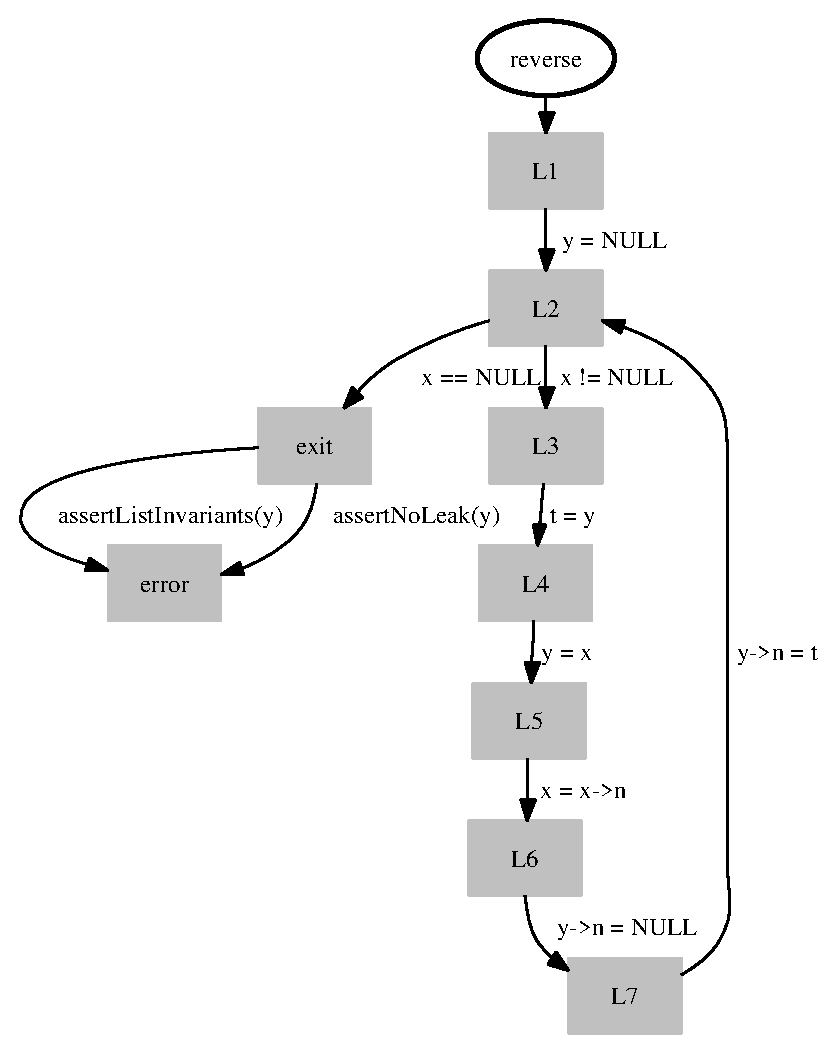
\epsfig{file=reverse_cfg,width=2.8in,height=3.0in}
\end{minipage}
\caption{\label{Fi:ManRevCFG}The CFG part of the TVP for the reverse function
shown in \figref{Reverse} and its corresponding CFG.}
\end{figure}


The specification of the analysis including the control flow graph
of the analyzed program is given in a format called TVP (Three
Valued Program). A TVP file should end with the extension '.tvp'.
The TVP for the analysis of the reverse function is given in
Figures \ref{Fi:ManRevDecl}, \ref{Fi:ManRevActions}, and
\ref{Fi:ManRevCFG}. The syntax of a TVP file is given in
\figref{TVPSyntax} and \figref{TVPSyntax2}. The syntax is in extended BNF when A $\bowtie$
B denotes a (possibly empty) sequence of A's separated by B's.

\begin{figure}
\framebox{
\begin{tabular}{ll}
\begin{minipage}[t]{1in}
\begin{tabbing}
\param{tvp} ::= \=\param{decl}$^*$ \seperator\ \param{action}$^*$ \seperator\ \\
\>\param{cfg\_edge}$^*$ \lb\seperator \csep{\param{cfg\_node}}\rb\\
\param{decl}\ \=\+::= \tvset\ \pid\ \param{set\_expr}\\
$|$ \predicate\=\ \ppred\ {\blp\ \csep{\pvar} \brp} \param{prop}$^*$\\
$|$ \instrum\=\ \ppred\ {\blp\ \csep{\pvar}\brp}\\
\>\bassign\/\ \pformula\ \param{flags}\\
$|$ \constraint\ \pformula\ \impliesT\ \pformula\\
$|$ \foreach\ \blp \param{iterator}\brp\ \blcb\ \param{decl}$^*$ \brcb\-\\
\ppred ::= \pid \lb\ \blb\ \csep{\pid}\ \brb\ \rb\\
\param{display} ::= \blcb\csep{\param{kleene}}\brcb\\
\param{iterator} ::= \pid\ \inset\ \param{set\_expr}\\
\param{kleene} ::= \textbf{1} $|$ \textbf{0} $|$ \textbf{1/2}\\
\param{action}\ \=\+::= \action\ \pid\ \blp\ \csep{\pid}\ \brp\ \blcb\\
    \lb\tvtitle\ \param{message}\rb\\
    \lb\focus\ \blcb\ \csep{\pformula}\rb\\
    \lb\precond\ \pformula\rb\\
    (\tvmessage\ \pformula\ {\bf \deref}\ \param{message})$^*$\\
    \lb\new\  \lb \pformula \rb\\
    \lb\blcb\ \param{update}$^*$\ \brcb\rb\\
    \lb\retain\ \pformula\rb \brcb\\
    (\tvmessage\ \pformula\ {\bf \deref}\ \param{message})$^*$\-\\    
\param{message}\ ::= (\param{quoted\_string}$|$\ppred)$\bowtie$\textbf{+}\\
\param{set\_expr}\ \=\+::= \param{set\_name}
$|$ \blcb\ \csep{\pid}\ \brcb\\
$|$ \param{set\_expr} \textbf{-} \param{set\_expr}\\
$|$ \param{set\_expr} \textbf{+} \param{set\_expr}\-\\
\param{update} ::=\=\ \ppred\ \blp\ \csep{\pvar}\ \brp\ \textbf{=} \pformula\\
\>$|$ \foreach\ \blp \param{iterator}\brp\ \blcb\ \param{update}$^*$ \brcb\\
\param{cfg\_edge} ::=\=\ \param{cfg\_node}\\
\>\pid\ \blp\ \csep{\pid}\ \brp\ \param{cfg\_node}\\
\end{tabbing}
\end{minipage}
&
\begin{minipage}[t]{1in}
\begin{tabbing}
// TVP file\\
\\
// Set declaration\\
// Core predicate\\
// Instrumentation predicate\\
\\
// Consistency rule\\
// For each id in the iterator\\
// Predicate name\\
// Predicate's flags\\
// Set iterator\\
// Functional dependencies\\
// Atomic values\\
// Action declaration\\
// Action title\\
// Focus formulae\\
// Precondition\\
// Report pre messages\\
// New individual(s)\\
// Update formulae\\
// Retain formula\\
// Report post messages\\
// Message for user\\
// Set definition\\
// Set difference\\
// Set union\\
// Update formula\\
// For each id in the iterator\\
// CFG edge\\
\end{tabbing}
\end{minipage}
\end{tabular}
}
\caption{\label{Fi:TVPSyntax}The syntax of a TVP file, part 1.}
\end{figure}

\begin{figure}
\framebox{
\begin{tabular}{ll}
\begin{minipage}[t]{1in}
\begin{tabbing}
\pformula\ \=\+::= \pformula\ \band\ \pformula\\
$|$ \pformula\ \bor\ \pformula\\
$|$ \pformula\ {\bf \deref} \pformula\\
$|$ \pformula\ {\bf {\tt <->}} \pformula\\
$|$ \bnot\pformula\\
$|$ \blp\pformula\=\ \textbf{?} \pformula\ \textbf{:} \pformula\brp\\
$|$ \var\ \beq\ \var\\
$|$ \var\ \bneq\ \var\\
$|$ \textbf{A}\nvars \pformula\\
$|$ \textbf{E}\nvars \pformula\\
$|$ \ppred\nvars\\
\\
$|$ \ppred\textbf{+}\twovars\\
\\
$|$ \ppred\textbf{*}\twovars\\
\\
$|$ \textbf{TC}\= \twovars\ \\
               \> \twovars\ \pformula\\
$|$ \param{kleene}\-\\
\end{tabbing}
\end{minipage}
&
\begin{minipage}[t]{1in}
\begin{tabbing}
// logical $\land$\\
// logical $\lor$\\
// logical implication\\
// logical equivalence\\
// logical $\neg$\\
// if-then-else\\
// equality\\
// inequality\\
// $\forall v_1, v_2, \ldots, v_n$\\
// $\exists v_1, v_2, \ldots, v_n$\\
// Predicate (of arbitrary\\
// arity)\\
// Transitive closure on \\
// binary predicate\\
// Reflexive and transitive \\
// closure on binary predicate\\
// Transitive closure on a\\
// general binary formula\\
// Atomic values\\
\end{tabbing}
\end{minipage}
\end{tabular}
}
\caption{\label{Fi:TVPSyntax2}The syntax of a TVP file, part 2 --- formulae.}
\end{figure}

\subsection{Predicates}
\label{Se:Predicates}

The predicate name can be either \pid\ or
\pid\blb\pid,~\ldots,~\pid\brb.
These are ordinary names.
The intention of the \pid\blb\pid,~\ldots,~\pid\brb\ format is to denote predicates which are
parameterized by source properties such as names of fields and pointer variables.
This is especially good for instrumentation predicates.
The predicate's arity is
determined by the number of variables in parenthesis.
%(currently the names of the variables are of no consequence).
For a description of the properties that can be used in predicate
declaration see \tableref{Prop}.

%%%%%%%%%%%%%% Display flags have been moved to proprty files %%%%%%%%%%%%%%%%%%%
%The \param{display} flag controls which values of the predicate are shown in the
%graph (in DOT).  The default is \{$1$, $1/2$\} specifying that true and unknown
%values are to be shown.
%%%%%%%%%%%%%%%%%%%%%%%%%%%%%%%%%%%%%%%%%%%%%%%%%%%%%%%%%%%%%%%%%%%%%%%%%%%%%%%%%

Instrumentation predicates are declared very similarly to core
predicates.  They use the same naming mechanism and the same flag
specification.  The only difference is that for an instrumentation
predicate the user has to attach its defining formula. The
formula's free variables should match the variables given in the
parenthesis (with the exception of precondition free variables
explained later).

\begin{table}
\begin{center}
\begin{tabular}{|l|l|l|l|}
\hline\hline
{\bf Property}  & {\bf Arity} & {\bf Meaning}   & {\bf Consistency Rule}\\
\hline \unique         & unary         & true for &
p(v1) \band\ p(v2) \impliesT v1 \beq\ v2\\
                &               & at most  &
E(v1) p(v1) \band\ v1 \bneq\ v \impliesT \bnot p(v)\\
                &               & one node & \\
\hline \function       & binary        & partial &
E(v) p(v, v1) \band\ p(v, v2) \impliesT v1 \beq\ v2\\
                &               & function &
E(v) p(v1, v) \band\ v2 \bneq\ v \impliesT \bnot p(v1, v2)\\
\hline \invfunction    & binary        & inverse of &
E(v) p(v1, v) \band\ p(v2, v) \impliesT v1 \beq\ v2\\
                &               & a partial &
E(v) p(v, v2) \band\ v1 \bneq\ v \impliesT \bnot p(v1, v2)\\
                &               & function &\\
\hline \symmetric      & binary        & &
p(v1, v2) \impliesT p(v2, v1)\\
\hline \antisymmetric  & binary        & &
p(v1, v2) \band\ p(v2, v1) \impliesT v1 \beq\ v2\\
                &               & &
p(v1, v2) \band\ v1 \bneq\ v2 \impliesT \bnot p(v2, v1)\\
\hline \reflexive      & binary        & &
v1 \beq\ v2 \impliesT p(v1, v2)\\
\hline \antireflexive  & binary        & &
v1 \beq\ v2 \impliesT \bnot p(v1, v2)\\
\hline \transitive     & binary        & &
E(v2) p(v1, v2) \band\ p(v2, v3) \impliesT p(v1, v3)\\
\hline \hline
\textbf{abs}    & unary         & $p$ is an     & N/A \\
                &               & abstraction   &\\
                &               & predicate     &\\
\hline
\textbf{nonabs} & unary         & $p$ is not an & N/A \\
                &               & abstraction   &\\
                &               & predicate     &\\
\hline
%\textbf{box}    & unary         & display $p$ & N/A \\
%                &               & in a box &\\
\hline \hline
\end{tabular}
\end{center}
\caption{\label{Ta:Prop}Properties of predicate p, their meaning
and the generated consistency rules.}
\end{table}

\subsection{\label{Se:FormulaeMan}Formulae}

The formula is evaluated in the context of a three valued logical
structure using the semantics of Kleene's $3$-valued logic.
Transitive closure of a general binary formula works as follows,
the last pair of variables are the free variables of the
subformula, and the first pair of variables are the variables of
the resulting TC relation.  The formula $\varphi_{cond} ?
\varphi_{true} : \varphi_{false}$ is an if-then-else formula. If
$\varphi_{cond}$ evaluates to true the value of the formula is
$\varphi_{true}$. If $\varphi_{cond}$ evaluates to false the value
of the formula is $\varphi_{false}$. If $\varphi_{cond}$ is
unknown then the result is the join of the values of
$\varphi_{true}$ and $\varphi_{false}$, i.e., the value of
$\varphi_{true}$ when it is equal to the value of
$\varphi_{false}$ and unknown otherwise.

\subsection{Consistency rules}

Most of the needed consistency rules for an analysis are
automatically generated from the functional properties of
predicates (see \tableref{Prop}) and from the instrumentation
predicates' defining formulae.  Sometimes it is useful to write
explicit consistency rules.  The left hand side of a consistency
rule (the body) is a general formula, the right hand side (the
head) is either an atomic formula or the negation of an atomic
formula, \impliesT stands for $\triangleright$.  Note that the
free variables of the body must match the free variables of the
head exactly.  A consistency rule state that for each assignment
to the free variables of the body that evaluate the body to $1$,
the head should also evaluate to $1$.  The action performed in
case of a consistency rule breach (i.e., the body of the
consistency rule is evaluated to $1$ and the head to $0$ or $1/2$
for a certain assignment) depends on the head of the consistency
rule as seen in \tableref{ConsAct}.
\begin{table}
\begin{center}
\begin{tabular}{|l|l|l|}
\hline \hline
\textbf{Head} & \textbf{Condition} & \textbf{Result}\\
\hline
0 & & The structure is invalid - discard.\\
\hline
1 & Never breached. & \\
\hline predicate & The value of the predicate for the &
The structure is invalid - discard.\\
          & assignment is false & \\
          & The value of the predicate for the & Coerce it to true.\\
          & assignment is unknown & \\
\hline
negated   & The value of the predicate for the & The structure is invalid - discard.\\
predicate & assignment is true & \\
          & The value of the predicate for the & Coerce it to false.\\
          & assignment is unknown & \\
\hline
variable & The two variables are assigned & The structure is invalid - discard.\\
equality         & to different nodes & \\
         & The variables are assigned to the & Coerce into a non summary node.\\
         & same node and it is a summary node & \\
\hline
variable  & The two variables are assigned & The structure is invalid - discard\\
inequality & to the same node & \\
\hline
\end{tabular}
\end{center}
\caption{\label{Ta:ConsAct}Result of a consistency rule breach
according to its head.}
\end{table}

\subsection{Actions}

The arguments of an action are predicate names\footnote{the
arguments can also include identifiers that are used to define
predicates.}  that can be used in the following formulae and will
be replaced with the actual arguments when the action is used (see
Section \ref{Se:CFGMan}). The actions section of the reverse
program is given in \figref{ManRevActions}.

\subsubsection{Specifying the title of an action with \tvtitle}
The title of the action, used when printing the action's
structures.

\subsubsection{Updating predicates}

Update formulae describe how predicates are updated as a result of
an action. If a predicate does not have an update formula then its
value before the action is retained. The formula is evaluated on
the old structure with the exception that nodes and predicates
added in the \new\ declaration are available. Note that update
clauses are not comma separated.

\subsubsection{Using preconditions for filtering with \precond} The
precondition formula is evaluated to check whether this action
should be performed.  If the formula is closed then a result of
true or unknown triggers the application of this action.  If the
formula contains free variables then the action is performed for
each assignment into these variables potentially satisfying the
formula.  The free variables can be used in the following formulae
and have the expected assignment.

\subsubsection{Focusing structures with \focus} The focus
formulae for this action. Applied before the precondition.

\subsubsection{Reporting messages with \tvmessage}
Messages that are reported to the user if the formula given is
potentially satisfied.

\subsubsection{Creating new nodes with \new}

An optional unary formula can be supplied. If no formula is
supplied then a single new node is created. If a formula is
supplied then each node potentially satisfying the formula is
duplicated, a new temporary binary predicate called $instance$ is
created matching the old node with the new node. In both cases an
unary predicated called $isNew$ is created an set true only for
the nodes created in this action. Both these predicates can be
used in the following formulae. The default value of all the
predicates when applied to the new nodes is false. If the unary
formula supplied evaluates to unknown for a certain node, the
matching new node becomes maybe active.

\subsubsection{Retaining nodes with \retain}

A mechanism for defining nodes that persist after an action. By
default, all nodes persist. This mechanism can be used to model
actions like free or even on-the fly garbage collection. An unary
formula must be supplied. Only nodes that potentially satisfy the
formula are retained. If the formulae supplied evaluates to
unknown for a certain node, it becomes maybe active instead of
being removed.

\subsection{\label{Se:CFGMan}Specifying the control flow graph}

The program to be analyzed is composed of CFG nodes with edges
connecting between them and actions to be performed on these
edges.  A flow insensitive analysis can be done by using a single
CFG node with actions on self loops.  A CFG node is declared
implicitly by the existence of incoming or outgoing CFG edges.
The action used in the CFG edge must be predefined in the actions
section.  The actual arguments passed to the action substitute the
formal arguments used in its definition.

If only a subset of the nodes should be printed the list of CFG
nodes to print should be supplied as the last section. The default
behavior is printing the structures available in each CFG node.


\subsection{Usability features}

TVP was designed to be written generically. Several constructs are
used to support this notion.

\subsubsection{Writing comments}

TVP supports C++ style comments: everything between /* and */ or
from // to the end of that line is ignored.

\subsubsection{Preprocessing}

The TVP file can be preprocessed using the standard C preprocessor
before being parsed by the system. The preprocessor enables file
inclusion (using the \#include directive), macro expansion (using
the \#define directive), and conditional evaluation (using the
\#if, \#endif, etc. directives).

\subsubsection{Sets}

Sets are a mechanism for grouping together several predicate names
to be used later in a \foreach\ clause or a composite formula. Set
operation such as union ($+$), and subtraction ($-$) can be used
to create set expressions.

\subsubsection{Foreach}

Sometimes a declaration, a focus formula or an update formula
should be repeated several times for different predicates, to
avoid code duplication TVP support the mechanism of \foreach. The
syntax is:

\noindent \begin{tabular}{l} \foreach\ \blp \pid\ \inset\
\param{set\_expr} \brp \blcb code \brcb
\end{tabular}

The code between the curly braces is duplicates once for each set
member and each time the predicate is substituted with the
appropriate set member.  Foreach can be applied to any declaration
(core predicate, instrumentation predicate, consistency rule), to
focus formulae and to update formulae in actions.

The \foreach\ mechanism can handle composite predicate names, in
this case only the identifiers within the square braces are
substituted.

\subsubsection{Composite operations}

Composite operations are a mechanism for applying a logical
operation (only \band\ and \bor\ are supported) on a set of
formulae.  This is similar to \foreach\ but can be used inside a
formula. The syntax is:

\noindent \begin{tabular}{l}
\param{op}/\{\pformula\ : \ppred\ \inset\ \param{set\_expr}\}
\end{tabular}

If the set is empty the neutral member for the operation is used
($0$ for \bor\ and $1$ for \band).  For example, the expression
\bor/\{$z$(v)~:~$z$~\inset~\{$x$,~$y$,~$t$\}~\} is expanded to
$x$(v)~\bor~$y$(v)~\bor~$t$(v).

\section{TVS}

The input structures for the analysis are described in a format
called TVS (Three Valued Structure). For example, the TVS for
input structure used in the analysis of the reverse function is
given in \figref{ManReverseTVS}. A TVS file name should end with
the extension '.tvs'. The syntax of a TVS file is given in
\figref{TVSSyntax}.

\begin{figure}
\framebox{
\begin{minipage}{1in}
\begin{tabbing}
\param{tvs} ::= \param{structure}$^*$\\
\param{structure} ::= \param{universe} \param{predicates}\\
\param{universe} ::= \textbf{\%n}\ \bassign\ \blcb\ \csep{\param{node}}\ \brcb\\
\param{predicates} ::= \textbf{\%p}\ \bassign\ \blcb\ \param{predicate}$^*$\ \brcb\\
\param{predicate} ::\=\+= \ppred\ \bassign\ \param{kleene} /* Nullary */\\
$|$ \ppred\ \bassign\ \blcb\ \csep{(\param{node} \lb\param{value}\rb)}\ \brcb\ /* Unary */\\
$|$ \ppred\ \bassign\ \blcb\
\csep{(\param{leftnode}\deref\param{rightnode}
\lb\param{value}\rb)}\ \brcb\ /* Binary */\\
$|$ \ppred\ \bassign\ \blcb\ \csep{(\csep{\pid})
\lb\param{value}\rb
}\ \brcb\ /* Arbitrary */\-\\
\param{node} ::=\+\=\ \pid\ \-\\
%%%%%%%%% -significant is no longer supported %%%%%%%%%%
%$|$ \blb\ \csep{\param{node}}\ \brb\\
%$|$ \param{node}\textbf{.}(\textbf{0}$|$\textbf{1})\-\\
%%%%%%%%%%%%%%%%%%%%%%%%%%%%%%%%%%%%%%%%%%%%%%%%%%%%%%%%
\param{value} ::= \textbf{:} \param{kleene}
\end{tabbing}
\end{minipage}
} \caption{\label{Fi:TVSSyntax}The syntax of a TVS file.}
\end{figure}

The value of a predicate defaults to false unless otherwise
specified in the TVS structure. All the node names used in the
predicates must be predefined. All the predicate names used must
be declared in the TVP file. If a node (or a node pair) is
specified without a value, the default of true (1) is taken. TVS
supports the same commenting style as TVP.

\newpage
\section{\label{Se:Command}Command line options}
\small
\begin{alltt}
Usage: tvla <program name> [input file] [options] Options:
 -d                      Turns on debug mode.
 -action [f][c]pu[c]b    Determines the order of operations computed
                         by an action. The default is fpucb.
                         f - Focus,  c - Coerce, p - Precondition.
                         u - Update, b - Blur.
 -join [algorithm]       Determines the type of join method to apply.
                         rel  - Relational join.
                         part - Partial join.
                         conc - No abstraction (i.e., blurring) is applied.
 -ms <number>            Limits the number of structures.
 -mm <number>            Limits the number of messages (default=0).
 -save {back|ext|all}    Determines which locations store structures.
                         back - at every back edge (the default).
                         ext  - at every beginning of an extended block.
                         all  - at every program location.
 -noautomatic            Supresses generation of automatic constraints.
 -props <file name>      Can be used to specify a properties file.
 -log <file name>        Creates a log file of the execution.
 -tvs <file name>        Creates a TVS formatted output.
 -dot <file name>        Creates a DOT formatted output.
 -tr:tvs <file name>     Creates a transition relation output in tvs-like format.
 -tr:dot <file name>     Creates a transition relation output in dot format.
 -D<macro name>[(value)] Defines a C preprocessor macro.
 -terse                  Turns off on-line information printouts.
 -nowarnings             Causes all warnings to be ignored.
 -path <directory path>  Can be used to specify a search path.
 -post                   Post order evaluation of actions.
\end{alltt}

\begin{itemize}
\item{\textbf{Analysis engine}}\\
Three different types of engines are available : \textbf{tvla} is
the classic chaotic iteration algorithm and the default one,
\textbf{tvmc} is a multithreading engine that performs a
state-space exploration using a search stack, and \textbf{ddfs} is
a Double-DFS multithreading engine that utilizes Buchi automata.

\item{\textbf{Backward Analysis}}\\
Some analyses need to propagate information in the opposite
direction specified for the CFG edges. To reverse the direction of
the CFG edges use the \textbf{-backward} flag. When this option is
chosen, the input structures are stored in the last location
computed by the topological sorting of the program locations.

\item{\textbf{Order of action evaluation}}\\
The default order of evaluation in the iterative algorithm is
reverse post order. However, when the analysis is very time/space
consuming and you want to see the structures that reach the end of
the analyzed program as soon as possible, use the \textbf{-post}
flag to use post order and get the desired effect.

\item{\textbf{Debugging}}\\
When debugging a new analysis it is useful to see the analysis as
it progresses and not just its final result. Use the \textbf{-d}
flag to see the structures in the different phases of execution.
In debug mode all the consistency rules are printed together with
their dependencies and each time a structure is discarded because
of an irreparable consistency rule breach, the problematic
consistency rule, assignment and structure are shown. Notice that
this mode generates very large PostScript files so you would
probably want to use the \textbf{-ms} flag.

\item{\textbf{Computing the effect of an action}}\\
Sometime you want to try and run the algorithms (Coerce, Focus,
Precondition, Update, Blur) in a different order or quantity than
the default one (Focus, Coerce, Precondition, Update, Coerce,
Blur). Use the \textbf{-action
\param{seq}} flag to control the computation of the action's
effect.  The argument is of the form [f][c]pu[c]b when: f - Focus,
c - Coerce, p - Precondition, u - Update, b -
Blur. % blur is now mandatory

\item{\textbf{Join method}}\\
Three join methods are available. To use the relational analysis
approach where (bounded) structures kept up to isomorphism choose
the \textbf{rel} option. To use the single-structure method use
the \textbf{ind} option. In this approach all the structures in a
CFG node that match with their nullary predicates' values are
merged into a single structure. The option is very useful for
analyses that would otherwise take a very long time and create
many structures. It is worth considering the \textbf{-action
fcpucb} specification when working in single structure mode. A
compromise between the two approaches merges structures that
identify on their nullary abstraction values and set of canonical
node names, thus considering only a partial set of predicates. To
use this option choose the \textbf{part}.  TVLA can perform
analysis without applying abstraction (i.e., blurring) via the
\textbf{conc} option.  This option can yield a
non-terminating analysis and therefore the \textbf{-ms} is usually
needed to force termination.

\item{\textbf{Maximum number of structures}}\\
A complex analysis may take a very long time and especially in
debug time may run forever. To see a partial result, you can limit
the number of structures generated using the \textbf{-ms
\param{number}} flag.

\item{\textbf{Maximum number of messages}}\\
The number of messages reported by the system can be limited. This
can be used to supply a condition that if holds the system stops
(by limiting the number of messages to $1$).

\item{\textbf{Saved locations}}\\
The default behavior of the system is to perform a join, and save
all the structures that reached the program location, only in
every back edge in the control graph (approximately once in every
loop). Saving structures at every program location is the most
efficient in terms of the number of structures generated (use
\textbf{-save all}). However, it is very space consuming. For a
compromise between the two extremes use \textbf{-save ext} which
saves structures only at the beginning of each extended block
(i.e., at every merge point in the control graph).

\item{\textbf{No automatic constraint generation}}\\
Sometimes it is useful to supply all the constraints by hand
without the automatically generated constraints. To do this supply
the \textbf{-noautomatic} flag.

\item{\textbf{Properties file}}\\
A properties file name can be supplied with the \textbf{-props}
option. The file is loaded before the analysis starts and
overrides all other property files. For more information see
section~\ref{Se:PropertyFiles}.

\item{\textbf{Log file}}\\
A log file name can be supplied with \textbf{-log} option. In this
case the majority of the information written to the console is
redirected to the log file.

\item{\textbf{TVS output file}}\\
A TVS output file name can be supplied with the \textbf{-tvs}
option. In this case the output of the analysis in TVS format is
directed to the file.

\item{\textbf{DOT output file}}\\
A DOT output file name can be supplied with the \textbf{-dot}
option. In this case the output of the analysis in DOT format is
directed to the file. The activation scripts for TVLA use this
option to create an output file for DOT by adding the `.dt'
extension to the program name. This option can be used to specify
a different file name for DOT, but the Postscript output should
then be created manually (the dotps script, supplied with TVLA,
can be used for this).

% This option is no longer supported
%\item{\textbf{Dumping intermediate results}}\\
%Some of the analyses can take a very long time. To see
%intermediate results the \textbf{-dump} flag can be used. The
%number supplied is the number of structures generated between
%each dump of the current set of structures per program location.

\item{\textbf{On-line information}}\\
TVLA reports information as the analysis progresses to the
standard output. To avoid seeing this information use the
\textbf{-terse} flag.

\item{\textbf{Preprocessor macros}}\\
Preprocessor macros can be passed to the parsers by using the\\
\textbf{-D$<$macro$>$(value)} option. This has the same effect
as\\
\verb"#define symbol value". For example, specifying -DCONCRETE
defines the CONCRETE symbol, and -DLEVEL(1) sets the value 1 to
the symbol LEVEL.

\item{\textbf{Search path}}\\
The option \textbf{-path} can be used to add directories to the
search path.

%%%%%%%%%%%%%%%%%%%%%%%%%%%%% Moved to property files %%%%%%%%%%%%%%%%%%%%%%%%%%%%
% \item{\textbf{Blur}}\\
% Two rules are implemented when determining which node
% should remain distinguished in the blur.  The default is two nodes must be
% different in the value of at least one abstraction predicate.  The second is two
% nodes must be different in a \emph{definite} value of at least one abstraction
% predicate.  Use the \textbf{-b2} flag to use the second rule.
%%%%%%%%%%%%%%%%%%%%%%%%%%%%%%%%%%%%%%%%%%%%%%%%%%%%%%%%%%%%%%%%%%%%%%%%%%%%%%%%%%

%%%%%%%%%%%%%%%%%%%% -significant is no longer supported %%%%%%%%%%%%%%%%%%%%%%%%%
%\item{\textbf{Node names}}\\
%It may be useful to track the nodes themselves
%from the original structures and during the different actions. Use the
%\textbf{-significant} to try and keep the names of the nodes significant. A
%materialization creates two nodes \param{node}.0 and \param{node}.1 according to
%the focused value of the predicate in question.  A blur that causes merging of
%nodes names the new nodes [\param{node},\ldots,\param{node}].  However, the
%nodes allocated by the new operation new node names in the
%form m\param{number}. In complex analyses using significant names may create
%very large names that create unreadable graphs.
%%%%%%%%%%%%%%%%%%%%%%%%%%%%%%%%%%%%%%%%%%%%%%%%%%%%%%%%%%%%%%%%%%%%%%%%%%%%%%%%%%
\end{itemize}

\section{Property files}
\label{Se:PropertyFiles}

A mechanism alternative to command-line options is available by
the means of property files. Property files consist of key-value
pairs using the syntax key=value. (More information about the
syntax of property files is available from the JDK documentation
of the java.util.Properties
class\footnote{\url{http://java.sun.com/j2se/1.4.2/docs/api/java/util/Properties.html}}.)
Each command-line option has a corresponding property.

There are several ways to pass properties to TVLA:
\begin{enumerate}
\item When TVLA is activated a tvla.properties file, which is
located at the installation directory is loaded. This file
contains all available properties and also includes documentation
for each.

\item Though it is possible to edit the tvla.properties file, it
is not recommended, because later TVLA versions may update this
file and also because this global change will affect every run of
TVLA.
%
If global changes are intended, add the properties that should be
change to the user.properties file, which is also located at the
installation directory. The properties in this file override the
ones in the tvla.properties file.

\item By creating a file with the same name as the program file
and the .properties extension (for example merge.properties for
merge.tvp) the properties in this file will load when this program
is used and override the ones passed by the previous methods.

\item By specifying a properties file name with the -props
command-line option. The properties in this file will override all
properties specified with the previous methods.

%\item By passing properties from the Java invocation line of TVLA.
%These properties will be overridden by properties specified by all
%other methods.

\item Finally, command-line options change their corresponding
properties and override properties specified by all other methods.
\end{enumerate}

Although all command-line options have corresponding properties,
there are other properties which do not correspond to command-line
options.  These are used to control TVLA behaviors which are less
common and also to test features as they are being developed.

%\section{TVLA Semantics}
\label{Se:TVLASemantics}

This section defines a formal semantics for TVLA actions.

%\section{Advanced Analysis Features}
\label{Se:TVLA_Analysis}


\subsection{Focus}

\subsection{Coerce}

\subsection{Update}

\subsection{Blur}

%\section{Additional Tools}



\subsection{Counterexample generation}


\subsection{Java Frontend}

\section{Additional references}

The TVLA system (version 0.9) was originally described in
\cite{kn:TalSAS00}.

The TVLA framework is described in \cite{TOPLAS:SRW02} and is a
good place to start understanding the theory behind the system.

%\section{Credits}

We would like to acknowledge the following people for contributing
to TVLA:
\begin{description}
    \item[Gilad Arnold:]
    \item [Ronald Biber:]
    \item[Nurit Dor:]
    \item [Guy Erez:]
    \item[John Field:]
    \item [Denis Gopan:]
    \item[Deepak Goyal:]
    \item [Hanne and Flemming Nielson:] 
    \item [Viktor Kuncak:]
    \item[Tel Lev-Ami:] For the design of the TVLA algorithms and the creation of the original 0.91 version.
    \item[Alexey Loginov:]
    For implementation of the Differencing feature and various coding
    contributions.
    \item [Ann Mulhern:]
    \item[Ganesan Ramalingam:]
    For re-designing the TVLA core and implementation of the
    functional representation algorithms.
    \item[Thomas Reps:]
    \item[Noam Rinetzky:]
    \item[Ran Shaham:]
    \item [Alex Warshavsky:]
    \item[Reinhard Wilhelm:]
    \item[Eran Yahav:]
    For implementation of the multi-threading engines (TVMC),\\
    various coding contributions.
    \item[Greta Yorsh:]
\end{description}


\newpage
\addcontentsline{toc}{section}{References}
\bibliographystyle{alpha}
\bibliography{tvla_references}

\appendix
\section{Changes since version 0.91}

The following changes are incorporated:
\begin{itemize}
\item Two multi-threading engines are now available for analyzing
multi-threaded programs. Currently, documentation for using them
is only available from
\url{http://www.cs.tau.ac.il/~yahave/3vmc.htm}.

%\item Many-sorted logics is supported with predicates of arbitrary
%order, see \secref{Predicates}. Type checking will be conducted.

\item A properties mechanism is added. This is described in
\ref{Se:PropertyFiles}.

\item The command-line options -b2 and -rotate have been moved to
property file.

\item The -significant option is no longer supported. This was
done in order to offer better performance by adding different
implementations for three-valued structures.

\item The -dump option is no longer supported.

\item The command-line option -join has been renamed to -save.

\item The command-line option -single has been replaced with the
-join option, which also includes a partial join (see the
command-line options section for more details).

\item The command-line option -action includes blur as a mandatory
operation, which is applied last.

\item The following command-line options are new :
%%-mode, -backward,
-props, -tvs, -dot, -D, -terse,  and -nowarnings. Consult the
command-line options sections before using them.

\item It is now possible to specify empty predicate update
sections.

\item Nullary predicates can be presented as either diamonds or
listed in a box. Use the tvla.dot.nullaryStyle property to choose
the desired presentation.

%\item Properties are used to control various the graphical
%representation of predicates, which are no longer part of the TVP
%specification. Use the tvla.dot.boxedPredicates to specify which
%predicates should be displayed in a box and the
%tvla.dot.displayedKleeneValues property to specify which Kleene
%values should be displayed for predicates.
\end{itemize}


\end{document}
